% !TeX root = ../main.tex
% Add the above to each chapter to make compiling the PDF easier in some editors.
\chapter{Concept}\label{chapter:Concept}
hier was dazwischen schreiben
viel technischer \newline
hough circles beschreiben etc.\newline\newline

The task of looking at a picture and telling what is in it, is quite trivial to humans and would usually not pose a challenging task to perform, whereas it is not that simple to Computers. In order to Classify images, or more exactly the objects comprised, machines ordinarily need a certain amount of Preprocessing to extract characteristic Features. As described in chapter \ref{chapter:Related Work} it is common practice to partition the many small steps of the process in two bigger, more generalized, steps of Feature Extraction and Classification. Our targeted devices are going to be any smartphones running Android as operating system, basically the App on the device should be able to handle live input from the Camera, detecting and classifying in real time. In the following subsections I am going to break down in detail, what  methods are used and how they work. \newline
Komponentendiagramm\newline
wieso nur bis 90? 

\section{Feature Extraction}
Before we pass data through to the Classification phase, it is a reasonable step in our Program, to specify a Region Of Interest, with regard to saving some processing power. In order to specify ROIs, I took advantage of the red circle around European Speed signs, the main steps of this part are to filter every red pixel out of the original image (\ref{fig:red_filtered_image}), subsequently an algorithm checks the filtered image for circles (\ref{fig:detected_image}). Filtering red pixels from a picture is not that big of a sorcery, so i am going to skip that part for now and come back later to this in the implementation section. The real magic happens when you try to search an image for circles, therefore a common method is the Circle Hough Transform. 
\subsection{Circle Hough Transform}
The Circle Hough Transform is a special case of the Hough transform, which determines lines in an image through Edge Detection Algorithms.


\begin{figure}[H]
	\minipage{0.33\textwidth}
	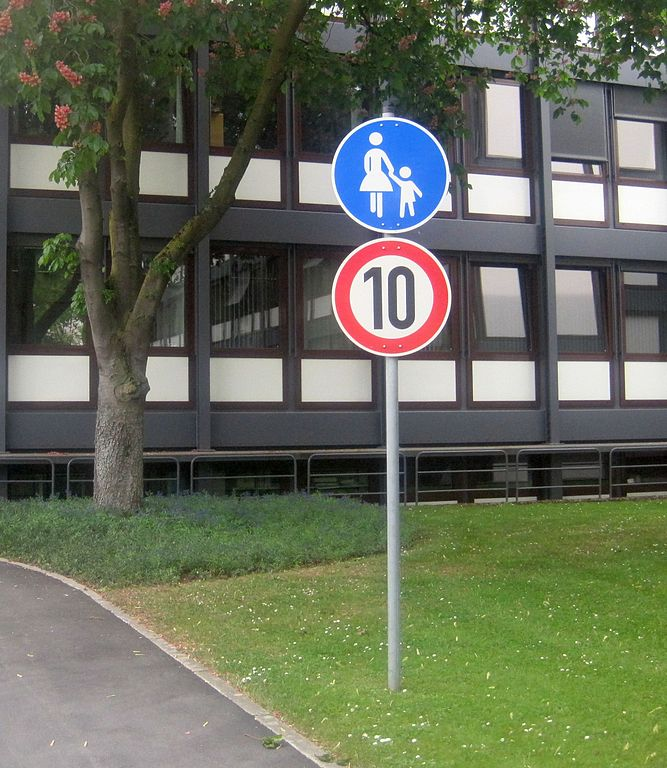
\includegraphics[width=\linewidth]{images/101.jpg}
	\caption{Original image}\label{fig:original_image}
	\endminipage\hfill
	\minipage{0.33\textwidth}
	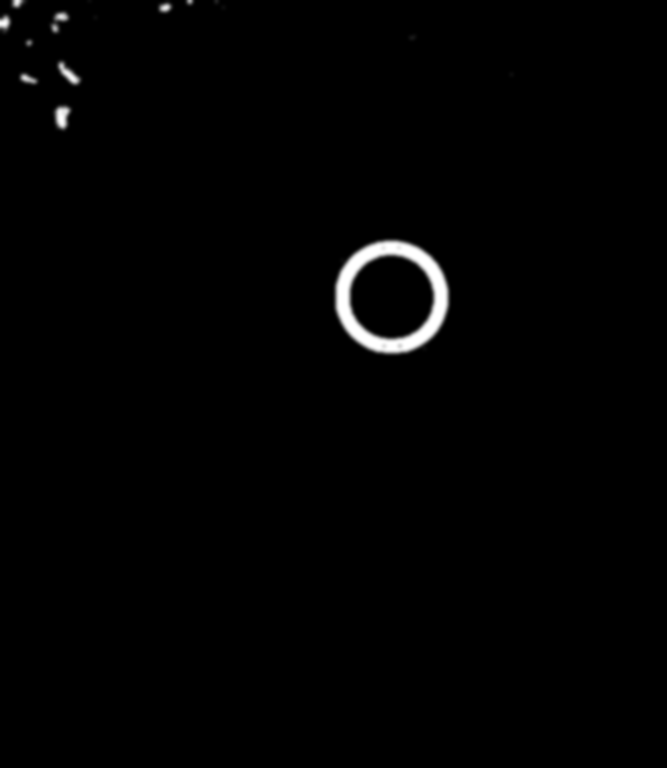
\includegraphics[width=\linewidth]{images/filteredimg.png}
	\caption{Filtered Image}\label{fig:red_filtered_image}
	\endminipage\hfill
	\minipage{0.33\textwidth}%
	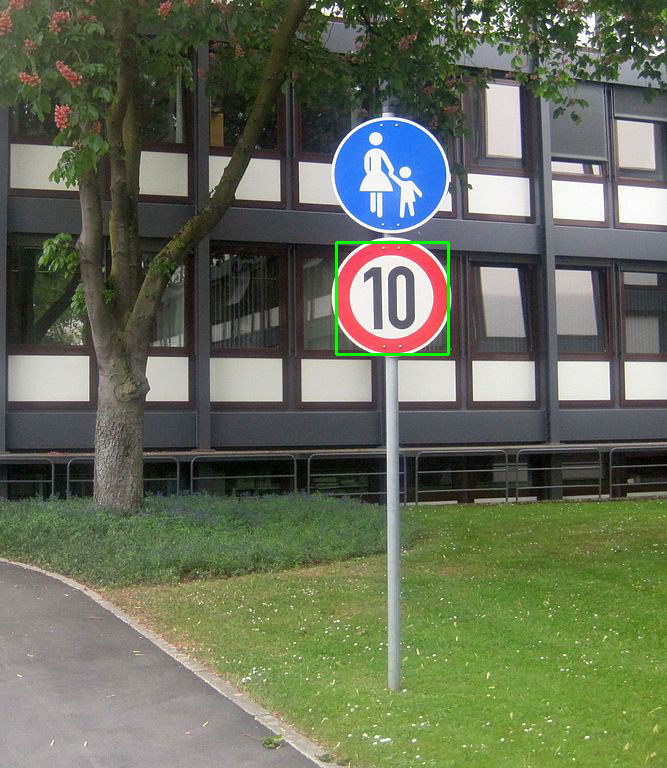
\includegraphics[width=\linewidth]{images/detectedimg.png}
	\caption{Detected image}\label{fig:detected_image}
	\endminipage
\end{figure}

\section{Classification}
Preceding stage delivers an image of fixed size, that needs to be categorized into one out of 10 groups, these are Speed limits "10km/h", "20km/h",..., "90km/h" and "no sign". To gain these information about the sub-image of the original image, I decided to apply a Feed Forward Deep Neural Network. Said Neural Network is fed each individual pixel, provided by the ROI to its input neurons, the trained Model then outputs a prediction on what class the input picture might belong to. 


Neuronales netz model